\documentclass[notitlepage]{problem-solving}

\author{Matt McCarthy}
\date{June 2016}
\title{Roots of Unity}

\usepackage{pgf,tikz}
\usepackage{mathrsfs}
\usetikzlibrary{arrows}

\definecolor{qqwuqq}{rgb}{0.,0.39215686274509803,0.}
\definecolor{xdxdff}{rgb}{0.49019607843137253,0.49019607843137253,1.}
\definecolor{qqqqff}{rgb}{0.,0.,1.}

\begin{document}

\maketitle

\begin{problem*}
	Factor the polynomial
	\[
		p=z^5-1.
	\]
\end{problem*}

\section{Background}

The complex numbers, denoted as $\CC$ are defined as follows.
\begin{definition}
	The set of \textit{complex numbers} is the following two-dimensional vector space over the real numbers.
	\[
		\CC := \set{a+bi\, :\, a,b\in\RR,\, i^2 = -1}
	\]
\end{definition}
\begin{figure}[h]
	\centering
	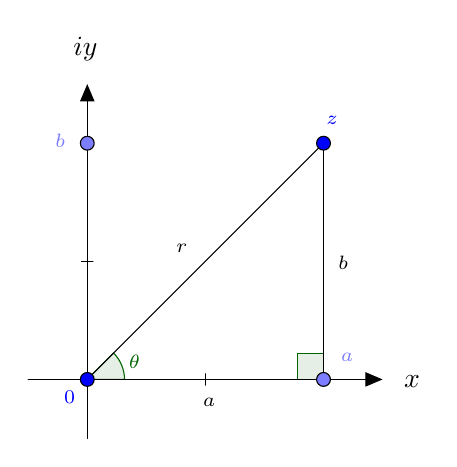
\begin{tikzpicture}[line cap=round,line join=round,>=triangle 45,x=1.5cm,y=1.5cm]
	\draw[->,color=black] (-0.5,0.) -- (2.5,0.);
	\foreach \x in {,1.,2.}
	\draw[shift={(\x,0)},color=black] (0pt,2pt) -- (0pt,-2pt);
	\draw[color=black] (2.6,-0.15) node [anchor=south west] {$x$};
	\draw[->,color=black] (0.,-0.5) -- (0.,2.5);
	\foreach \y in {,1.,2.}
	\draw[shift={(0,\y)},color=black] (2pt,0pt) -- (-2pt,0pt);
	\draw[color=black] (-0.2,2.8) node [anchor=west] {$iy$};
	\clip(-0.5,-0.5) rectangle (2.5,2.5);
	\draw[color=qqwuqq,fill=qqwuqq,fill opacity=0.1] (2.,0.22277768022923544) -- (1.7772223197707646,0.22277768022923547) -- (1.7772223197707646,0.) -- (2.,0.) -- cycle;
	\draw [shift={(0.,0.)},color=qqwuqq,fill=qqwuqq,fill opacity=0.1] (0,0) -- (0.:0.3150552167742013) arc (0.:45.:0.3150552167742013) -- cycle;
	\draw (0.,0.)-- (2.,2.);
	\draw (2.,2.)-- (2.,0.);
	\draw (0.,0.)-- (2.,0.);
	\begin{scriptsize}
	\draw [fill=qqqqff] (2.,2.) circle (2.5pt);
	\draw[color=qqqqff] (2.0719752655925316,2.191528364493368) node {$z$};
	\draw [fill=qqqqff] (0.,0.) circle (2.5pt);
	\draw[color=qqqqff] (-0.15,-0.15) node {$0$};
	\draw[color=black] (0.8012525579365867,1.109838786901943) node {$r$};
	\draw [fill=xdxdff] (2.,0.) circle (2.5pt);
	\draw[color=xdxdff] (2.2,0.185676817697619) node {$a$};
	\draw[color=black] (2.1664918306247922,0.9838167001922624) node {$b$};
	\draw [fill=xdxdff] (0.,2.) circle (2.5pt);
	\draw[color=xdxdff] (-0.22792781685913763,2.023498915547127) node {$b$};
	\draw[color=black] (1.0322930502376675,-0.19238944243142264) node {$a$};
	\draw[color=qqwuqq] (0.4,0.15) node {$\theta$};
	\end{scriptsize}
	\end{tikzpicture}
	\caption{A diagram of the complex plane.\label{c}}
\end{figure}
\noindent Furthermore, all $z\in\CC$ have a \textit{polar form}
\[
	z=r(\cos\theta+i\sin\theta)
\]
where $r,\theta\in\RR$ with $r\geq 0$.
Moreover, $\theta$ is called the \textit{argument} of $z$.
Additionally, we have Euler's formula which allows us to write the polar form of a complex number more concisely.
\begin{thm}
	For all $\theta\in\RR$,
	\[
		e^{i\theta} = \cos\theta+i\sin\theta.
	\]
\end{thm}
\noindent Thus, any $z\in\CC$ can be written as
\[
	z=re^{i\theta}.
\]
Moreover, for any $z=a+bi=re^{i\theta}\in\CC$, the \textit{modulus} of a $z$ is defined as
\[
	|z| := \sqrt{a^2+b^2} = r.
\]
Lastly, an \textit{$n$th root of unity} is a $z\in\CC$ such that
\[
	z^n = 1.
\]

\section{Solution}

\begin{problem*}
	Factor the polynomial
	\[
		p=z^5-1.
	\]
\end{problem*}

\noindent In order to factor $p$, we want to find the roots of the equation
\[
	z^5 - 1= 0.
\]
Equivalently, we will find the 5th roots of unity, or the solutions to
\[
	z^5 = 1.
\]
To begin, we know that $z=re^{i\theta}$ for some $r\geq 0$ and $\theta\in\RR$.
Furthermore, we know that $1=e^{2ki\pi}$ for all $k\in\ZZ$.
Thus,
\[
	r^5e^{5i\theta} = e^{2ki\pi}
\]
for all $k\in\ZZ$.
Since $|e^{i\phi}| = 1$ for all $\phi\in\RR$, we know that $r^5 = 1$.
Thus, $r=1$ because $r$ is a positive real.
Thus, we are left with
\[
	e^{5i\theta}=e^{2ki\pi}.
\]
Ergo,
\[
	\theta = 2ki\pi/5
\]
for all $k\in\ZZ$.
However, this is an infinite solution set and there are only 5 \textit{distinct} solutions.
To find these distinct solutions, we use the fact that
\[
	e^{i\theta} = e^{i(\theta+2k\pi)}
\]
for any $k\in\ZZ$.
Thus, our distinct values for $\theta$ are as follows.
\[
	\theta\in\set{0, 2\pi/5, 4\pi/5, 6\pi/5, 8\pi/5}
\]
When $\theta =10\pi/5 = 2\pi$, we get the same result as when $\theta=0$ since $2\pi\equiv 0\mod{2\pi}$.
Therefore,
\[
	z\in S:=\set{1,e^{2\pi/5}, e^{4\pi/5}, e^{6\pi/5}, e^{8\pi/5}}.
\]
Since each of the elements of the solution set is a root of the polynomial, $z^5-1$, we can factor out $z-r$ from $p$ for each $r\in S$.
Thus,
\[
	p = z^5-1=(z-1)(z-e^{2\pi/5})(z-e^{4\pi/5})(z-e^{6\pi/5})(z-e^{8\pi/5}).
\]

\end{document}
